\documentclass{article}
\usepackage[margin=1.0in]{geometry}
\usepackage{amsmath, amssymb, mathrsfs}
\usepackage[english]{babel}
\usepackage{graphicx}
\usepackage{pgfplots}
\pgfplotsset{width=10cm,compat=1.9}
\usepackage{enumerate}
\usepackage{tikz}
\usetikzlibrary{shapes,backgrounds}
\let\vec\mathbf


\title{Numerical Computing HW 7}
\author{Greg Stewart}
\date{\today}

\begin{document}

\maketitle

\section*{8.2 \normalsize Determine the least squares approximation of the form $f(x) = a + b\sin(x)$}

\begin{table}[h!]
  \centering
  \begin{tabular} {c | c c c }
    $x_i$ & $-\frac{\pi}{2}$ & 0 & $\frac{\pi}{6}$ \\ 
    \hline  
    $f_i$ & 2 & 0 & -1 \\
  \end{tabular}
\end{table}

The error function in this case is

$$E(a,b) = \sum_{i=1}^n (a + b\sin(x_i) - y_i)^2$$

which we need to minimize. Differentiating we get

$$\frac{\partial E}{\partial a} = 2\sum_{i=1}^n (a + b\sin(x_i) - y_i)$$
$$\frac{\partial E}{\partial b} = 2\sum_{i=1}^n (a + b\sin(x_i) - y_i)\sin(x_i)$$

And so we can write the normal equation

\[
  \begin{pmatrix}
    n & \sum_i \sin(x_i) \\ \sum_i \sin(x_i) & \sum_i \sin^2(x_i) \\
  \end{pmatrix}
  \begin{pmatrix}
    a \\ b \\
  \end{pmatrix}
  =
  \begin{pmatrix}
    \sum_{i} y_i \\ \sum_i y_i\sin(x_i) \\
  \end{pmatrix}
\]

And solve for $a$ and $b$.

\[
  \begin{pmatrix}
    a \\ b \\
  \end{pmatrix}
  =
  \frac{1}{n\sum_i \sin^2(x_i) - (\sum_i\sin(x_i))^2}
  \begin{pmatrix}
    \sum_i\sin^2(x_i) & -\sum_i\sin(x_i) \\ -\sum_i\sin(x_i) & n \\
  \end{pmatrix}
  \begin{pmatrix}
    \sum_i y_i \\ \sum_i y_i\sin(x_i) \\
  \end{pmatrix}
\]

\[
  \begin{pmatrix}
    a \\ b
  \end{pmatrix}
  =
  \begin{pmatrix}
    0 \\ -2
  \end{pmatrix}
\]

So the approximation is $f(x) = -2\sin(x)$.






\section*{8.5(b)-(d) \normalsize Elliptical path of a comet is described by}

$$r = \frac{p}{1 + \epsilon \cos \theta}$$

\begin{table}[h!]
  \centering
  \begin{tabular} {c | c c c c c }
    $\theta_i$ & 0.00 & 1.57 & 3.14 & 4.71 & 6.28 \\
    \hline
    $r_i$ & 0.62 & 1.23 & 16.14 & 1.35 & 0.62 \\
  \end{tabular}
\end{table}

\begin{enumerate}[(a)]\setcounter{enumi}{1}
  \item \textit{By writing the model function as follows, explain how the nonlinear regression problem can be trandormed into one with model function $R = V_1 + V_2\cos(\theta)$. Also, what happens to the data values?}

    $$\frac{1}{r} = \frac{1 + \epsilon\cos\theta}{p}$$

    Let $R = \frac{1}{r}$, $V_1 = \frac{1}{p}$, and $V_2 = \frac{\epsilon}{p}$. This gives the given form of the model function. None of the $\theta_i$ change, as they are still part of the model equation, but instead of using $r_i$, we use $R_i = \frac{1}{r_i}$.
  \item \textit{Writing the model function in part (b) as $R = G(\theta)$, and using the least squares error function, compute $V_1$ and $V_2$. Determine $p$ and $\epsilon$.}

    We have for the error function

    $$E(V_1,V_2) = \sum_{i=1}^n [V_1 + V_2\cos(\theta_i) - R_i]^2$$

    which we can differentiate to get
    $$\frac{\partial E}{\partial V_1} = 2\sum_{i=1}^n (V_1 + V_2\cos(\theta_i) - R_i)$$
    $$\frac{\partial E}{\partial V_2} = 2\sum_{i=1}^n (V_1 + V_2\cos(\theta_i) - R_i)\cos(\theta_i)$$

    And upon setting these to 0 we get the matrix equation
    
    \[
      \begin{pmatrix}
        n & \sum_i \cos(\theta_i) \\ \sum_i \cos(\theta_i) & \sum_i \cos^2(\theta_i) \\
      \end{pmatrix}
      \begin{pmatrix}
        V_1 \\ V_2 \\
      \end{pmatrix}
      =
      \begin{pmatrix}
        \sum_{i} R_i \\ \sum_i R_i\cos(R_i) \\
      \end{pmatrix}
    \]

    Which can be easily solved for $V_1$ and $V_2$
    
    \[
      \begin{pmatrix}
        V_1 \\ V_2 \\
      \end{pmatrix}
      =
      \frac{1}{n\sum_i \cos^2(\theta_i) - (\sum_i\cos(\theta_i))^2}
      \begin{pmatrix}
        \sum_i\cos^2(\theta_i) & -\sum_i\cos(\theta_i) \\ -\sum_i\cos(\theta_i) & n \\
      \end{pmatrix}
      \begin{pmatrix}
        \sum_i R_i \\ \sum_i R_i\cos(\theta_i) \\
      \end{pmatrix}
    \]

    \[
      \begin{pmatrix}
        V_1 \\ V_2
      \end{pmatrix}
      =
      \begin{pmatrix}
        0.83885 \\ 0.21575
      \end{pmatrix}
    \]

    And now we can solve for $p$ and $\epsilon$:

    \begin{align*}
      p &= \frac{1}{V_1} = 1.192 \\
      \epsilon &= pV_2 = 0.257 \\
    \end{align*}

    
    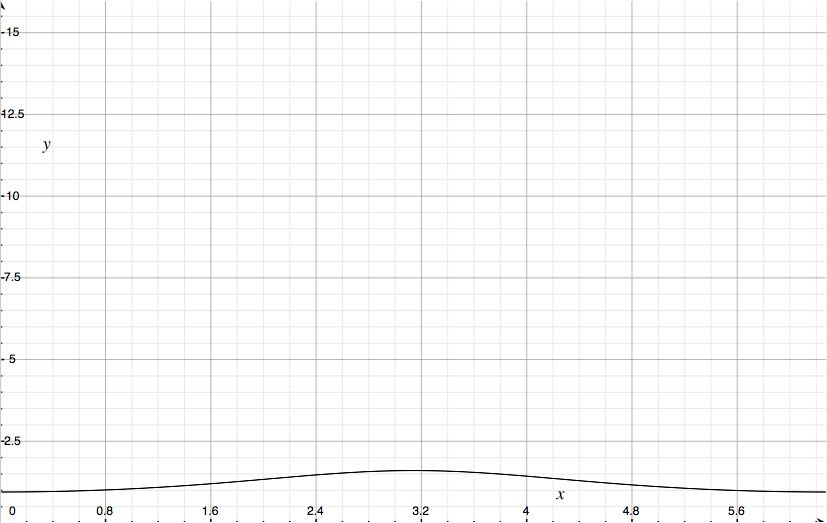
\includegraphics[width=\textwidth]{graph-c.jpg}
    
  \item \textit{Redo (c) but use the relative least squares error function:}

    $$E_R(V_1, V_2) = \sum_{i=1}^{n}\Big(\frac{G(\theta_i) - R_i}{R_i}\Big)^2$$

    Again, we need to differentiate and set to 0, which gets us

    $$\frac{\partial E}{\partial V_1} = 0 = V_1\sum\frac{1}{R_i^2} + V_2\sum\frac{\cos\theta_i}{R_i^2} - \sum\frac{1}{R_i}$$
    $$\frac{\partial E}{\partial V_2} = 0 = V_1\sum\frac{\cos\theta_i}{R_i^2} + V_2\sum\frac{\cos^2\theta_i}{R_i^2} - \sum\frac{\cos\theta_i}{R_i}$$

    And produces the matrix equation

    \[
      \begin{pmatrix}
        \sum\frac{1}{R_i^2} & \sum\frac{\cos\theta_i}{R_i^2} \\
        \sum\frac{\cos\theta_i}{R_i^2} & \sum\frac{\cos^2\theta_i}{R_i^2} \\
      \end{pmatrix}
      \begin{pmatrix}
        V_1 \\ V_2
      \end{pmatrix}
      =
      \begin{pmatrix}
        \sum\frac{1}{R_i} \\ \sum\frac{\cos\theta_i}{R_i}
      \end{pmatrix}
    \]

    Which allows us to solve for $V_1$ and $V_2$.

    \[
      \begin{pmatrix}
        V_1 \\ V_2
      \end{pmatrix}
      =
      \frac{1}{\sum\frac{1}{R_i^2}\sum\frac{\cos^2\theta_i}{R_i^2} - \sum\frac{\cos\theta_i}{R_i^2}\sum\frac{\cos\theta_i}{R_i^2}}
      \begin{pmatrix}
        \sum\frac{\cos^2\theta_i}{R_i^2} & -\sum\frac{\cos\theta_i}{R_i^2} \\
        -\sum\frac{\cos\theta_i}{R_i^2} & \sum\frac{1}{R_i^2}
      \end{pmatrix}
      \begin{pmatrix}
        \sum\frac{1}{R_i} \\ \sum\frac{\cos\theta_i}{R_i}
      \end{pmatrix}
    \]

    \[
      \begin{pmatrix}
        V_1 \\ V_1
      \end{pmatrix}
      =
      \frac{1}{1672.52299}
      \begin{pmatrix}
        1344.92834 \\ 1241.63015
      \end{pmatrix}
    \]
    \[
      \begin{pmatrix}
        V_1 \\ V_1
      \end{pmatrix}
      =
      \begin{pmatrix}
        0.80413 \\ 0.74237
      \end{pmatrix}
    \]

    And we use these values to calculate $p$ and $\epsilon$:

    \begin{align*}
      p &= \frac{1}{V_1} = 1.244 \\
      \epsilon &= pV_2 = 0.923
    \end{align*}
    
    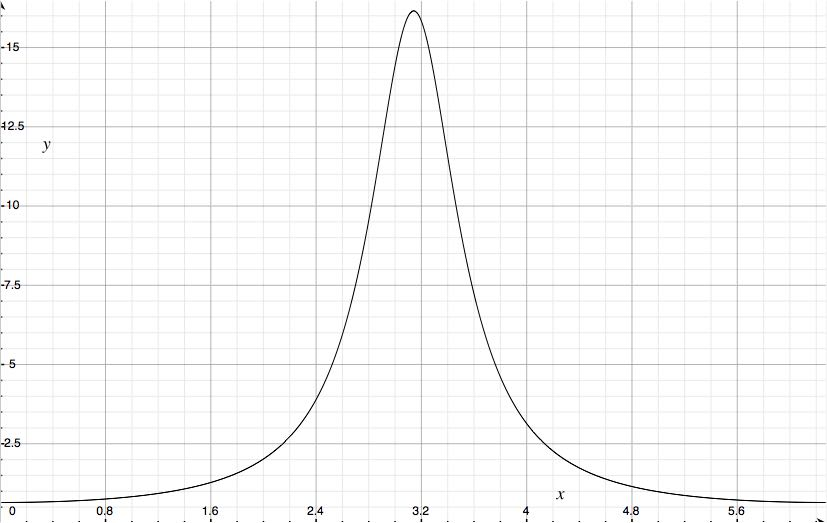
\includegraphics[width=\textwidth]{graph-d.jpg}


\end{enumerate}



\section*{8.12 \normalsize Consider the equation:}

\[
  \begin{pmatrix}
    3 & 1 \\ 1 & 2 \\
  \end{pmatrix}
  \begin{pmatrix}
    v_1 \\ v_2 \\
  \end{pmatrix}
  =
  \begin{pmatrix}
    1 \\ -1 \\
  \end{pmatrix}
\]

\begin{enumerate}[(a)]
  \item \textit{What is the quadratic form associated with this equation? Write it out as a polynomial.}

    $$F(\vec{v}) = \frac{1}{2}\vec{v}^T\vec{A}\vec{v}-\vec{b} \cdot \vec{v}$$

    \begin{align*}
      F(\vec{v}) &= \frac{1}{2}
      \begin{pmatrix}
        v_1 & v_2
      \end{pmatrix}
      \begin{pmatrix}
        3 & 1 \\ 1 & 2 \\
      \end{pmatrix}
      \begin{pmatrix}
        v_1 \\ v_2
      \end{pmatrix}
      -
      \begin{pmatrix}
        1 \\ -1
      \end{pmatrix}
      \cdot
      \begin{pmatrix}
        v_1 \\ v_2
      \end{pmatrix} \\
      &= \frac{1}{2}(3v_1^2 + 2v_1v_2 + 2v_2^2 - v_1 + v_2)
    \end{align*}

  \item \textit{In this question you are to use the SDM. Taking $\vec{v_1} = (-1,2)^T$, calculate $\vec{v_2}$.}

    We need $\vec{r_1}$, $\vec{q_1}$, and $\alpha_1$ to get $\vec{v_2}$.

    \[
      \vec{r_1} =
      \begin{pmatrix}
        1 \\ -1
      \end{pmatrix}
      -
      \begin{pmatrix}
        3 & 1 \\ 1 & 2 \\
      \end{pmatrix}
      \begin{pmatrix}
        -1 \\ 2
      \end{pmatrix}
      = 
      \begin{pmatrix}
        2 \\ -4
      \end{pmatrix}
    \]
    \[
      \vec{q_1} =
      \begin{pmatrix}
        3 & 1 \\ 1 & 2 \\
      \end{pmatrix}
      \begin{pmatrix}
         2 \\ -4
      \end{pmatrix}
      = 
      \begin{pmatrix}
        2 \\ -6
      \end{pmatrix}
    \]
    \[
      \alpha_1 = \frac{\vec{r_1} \cdot \vec{r_1}}{\vec{r_1} \cdot \vec{q_1}} = \frac{20}{28} = \frac{5}{7}
    \]

    With this we can get the next point:
    
    \[
      \vec{v_2} = \vec{v_1} + \alpha_1 \vec{r_1} =
      \begin{pmatrix}
        -1 \\ 2
      \end{pmatrix}
      + \frac{5}{7}
      \begin{pmatrix}
        2 \\ -4
      \end{pmatrix}
      =
      \begin{pmatrix}
        \frac{3}{7} \\ -\frac{6}{7}
      \end{pmatrix}
    \]

  \item \textit{In this question you are to use the CGM. Taking $\vec{v_1} = (-1,2)^2$, calculate $\vec{v_2}$ and $\vec{v_3}$.}

    For CGM, $\vec{v_2}$ is exactly the same as for SDM, so we have 

    \[
      \vec{v_2} = 
      \begin{pmatrix}
        \frac{3}{7} \\ -\frac{6}{7}
      \end{pmatrix}
    \]

    Which we can use to calculate $\vec{v_3}$. Using the formulae for $\vec{r_2}, \beta_1, \vec{d_2}, \vec{q_2},$ and $\alpha_2$ from the text, it's easy to obtain

    \begin{align*}
      \vec{r_2} &= \frac{1}{7}
      \begin{pmatrix}
        4 \\ 2
      \end{pmatrix} \\
      \beta_1 &= \frac{1}{49} \\
      \vec{d_2} &= \frac{1}{49}
      \begin{pmatrix}
        30 \\ 10
      \end{pmatrix} \\
      \vec{q_2} &= \frac{1}{49}
      \begin{pmatrix}
        100 \\ 50
      \end{pmatrix} \\
      \alpha_2 &= \frac{20}{1/49 (35000)} = \frac{98}{350} \\
      \vec{v_3} &= \vec{v_2} + \alpha_2\vec{d_2} \\
      &= \frac{1}{5}
      \begin{pmatrix}
        3 \\ -4
      \end{pmatrix}
    \end{align*}




\end{enumerate}






\section*{8.24 \normalsize Consider the following function, where $\vec{A}$ is a symmetric positive definite 2 $\times$ 2 matrix, and $\vec{v} = (v_1, v_2)^T$.}

$$F(\vec{v}) = \frac{1}{2} \vec{v}^T \vec{A} \vec{v} - \vec{b} \cdot \vec{v}$$

\begin{enumerate}[(a)]
  \item \textit{Shown is the starting point $\vec{v_1}$ and the point $\vec{v_2}$ calculated using the CGM. Determine where the next point $\vec{v_3}$ is located.}

    Since we're using CGM here, by theorem 8.2 in the text, we must come to a solution in $m \leq n+1$ steps. $n$ in this case is 2, so it can take a maximum of 3 steps to reach the minimum. Since we're on $v_2$ and only have one step left, we are left with the fact that $\vec{v_3}$ will in fact be at the minimum.  
  \item \textit{If one uses the same starting point for SDM, where is $\vec{v_2}$}

    Using SDM, $\vec{v_2}$ will be in the same spot as it is for the case of CGM, since in for $\vec{v_2}$ and \textit{only} $\vec{v_2}$, the formula for its calculation is the same in both CGM and SDM.
  \item \textit{What starting point $\vec{v_1}$ should be used so the point $\vec{v_2}$ computed by the SDM is exactly at the minimum?}

    To get it in one go, $\vec{v_1}$ must be on a contour which is orthognal to the direction of the minimum. Thus, it could be at approximately (4,2), or around (2.5, -4). Any of these type of points would work. 
\end{enumerate}






\section*{8.33 \normalsize Consider $\vec{A}\vec{x} = \vec{b}$, where $\vec{b} = \vec{A}\vec{x}$, $\vec{x} = (1,1,\dots,1)^T$, and $\vec{A}$ is the tridiagonal symmetric positive definite matrix as defined.}

\begin{enumerate}[(a)]
  \item \textit{Use MATLAB to fill out the table. $x_c$ is the solution computed using CGM. The computing time is how long it takes to execute the CGM algorithm.}

    \begin{table}[h!]
      \centering
      \begin{tabular} {c | c | c | c | c }
        $n$ & $\frac{||x-x_c||}{||x||_{\infty}}$ & $\kappa_{\infty}(A)$ & Number Iterations & Compute Time \\
        \hline
        100 & $1.3323\times 10^{-15}$ & 5000 & 52 & 0.009302s \\
        \hline
        500 & $5.3291\times 10^{-15}$ & $1.25\times 10^{5}$ & 254 & 0.034839s \\
        \hline
        1000 & $2.0761\times 10^{-14}$ & $5\times10^5$ & 505 & 0.221704s\\
        \hline
        2000 & $1.5321\times 10^{-14}$ & $2\times10^6$& 1009 & 1.114833s
      \end{tabular}
    \end{table}

  \item \textit{Based on your results, can you predict the number iterations when $n = 4000$? Computing time?}

    The number of iterations should be about 4000/2 = 2000, and based on the trends perhaps about 2014.

    The computing time should be on the order of about 10 seconds.
  \item \textit{Using MATLAB command $ones$, determine the smallest integer value of $k$ where MATLAB states there is an "Error using ones" and that the "array exceeds maximum array size preference." With this, run the CGM code with $n = (k-1)\cdot1000$ and report ont he value of $n$ you used, the number of iterations, and the computing time. Then, do this with $sparse(A)$, and report again.}

    
    The smallest $k$ in my case is 32, so I'll run CGM with $n = 32000$.

    Unfortunately, neither of the representations of $A$ led to anything close to a quick calculation, and I terminated the processes after a few minutes.
\end{enumerate}

















\end{document}
